\documentclass[10pt]{beamer}
\usefonttheme{professionalfonts,serif}
\def\newblock{\hskip .11em plus .33em minus .07em}
\usepackage[numbers,sort]{natbib}
\renewcommand{\rmdefault}{psbx}
\usepackage[utf8]{inputenc}
\usepackage[T1]{fontenc}
\usepackage{textcomp}
\usepackage{eulervm}

\usetheme{default}           % tips from David Blei
\useinnertheme{circles}
\useoutertheme{infolines}
\setbeamertemplate{headline}{}
\setbeamertemplate{navigation symbols}{}
\setbeamerfont{itemize/enumerate subbody}{size=\normalsize}
\setbeamerfont{itemize/enumerate subsubbody}{size=\normalsize}
\usecolortheme{seahorse}
\setbeamersize{text margin left=2mm,text margin right=2mm}

\graphicspath{{../../figures/}}

\definecolor{mypine}{rgb}{0.05,0.45,0.05}
\definecolor{mycyan}{rgb}{0.0,0.9,0.9}
\newcommand{\Red}{\textcolor{red}}
\newcommand{\Blue}{\textcolor{blue}}
\newcommand{\Green}{\textcolor{mypine}}
\newcommand{\PineGreen}{\textcolor{mypine}}
\newcommand{\Magenta}{\textcolor{magenta}}
\newcommand{\Cyan}{\textcolor{mycyan}}

\newcommand{\N}{\mathcal{N}}
\newcommand{\R}{\mathbb{R}}
\newcommand{\T}{{\scriptsize^{\top}}}
\newcommand{\D}{\mathcal{D}}
\newcommand{\F}{\mathcal{F}}
\newcommand{\E}{\mathbb{E}}
\newcommand{\V}{\mathbb{V}}
\newcommand{\M}{\mathcal{M}}
\newcommand{\KL}{\mathcal{KL}}
\newcommand{\cut}[1]{}
\newcommand{\trace}{\operatorname{trace}}

\newcommand{\bmu}{{\boldsymbol{\mu}}}
\newcommand{\btheta}{\boldsymbol{\theta}}
\newcommand{\bepsilon}{\boldsymbol{\epsilon}}
\newcommand{\balpha}{\boldsymbol{\alpha}}
\newcommand{\bbeta}{\boldsymbol{\beta}}
\newcommand{\bphi}{\boldsymbol{\phi}}
\newcommand{\bPhi}{\boldsymbol{\Phi}}
\newcommand{\bSigma}{\boldsymbol{\Sigma}}
\newcommand{\bpi}{\boldsymbol{\pi}}
\newcommand{\blambda}{\boldsymbol{\lambda}}

\newcommand{\argmax}{\operatorname{argmax}}
\newcommand{\argmin}{\operatorname{argmin}}
\newcommand{\ci}{{\bot\negthickspace\negthickspace\bot}} % conditional indep.
\newcommand{\neigh}{\operatorname{ne}}
\newcommand{\vectr}[2]{  \left[ \!\!\begin{array}{c} #1 \\
      #2 \end{array} \!\!\right]}
\newcommand{\deff}{\stackrel{\mathrm{def}}{=}}
\newcommand{\deldel}[2]{\frac{\partial #1}{\partial #2}}

\newcommand{\maketilde}{\raisebox{0.4ex}{\tiny $\sim$}}
\newcommand{\bfa}{\mathbf a}
\newcommand{\bfb}{\mathbf b}
\newcommand{\bfe}{\mathbf e}
\newcommand{\bff}{\mathbf f}
\newcommand{\bfk}{\mathbf k}
\newcommand{\bfm}{\mathbf m}
\newcommand{\bfn}{\mathbf n}
\newcommand{\bfp}{\mathbf{p}}
\newcommand{\bfs}{\mathbf s}
\newcommand{\bfu}{\mathbf u}
\newcommand{\bfx}{\mathbf x}
\newcommand{\bfy}{\mathbf y}
\newcommand{\bft}{\mathbf t}
\newcommand{\bfv}{\mathbf v}
\newcommand{\bfw}{\mathbf w}
\newcommand{\bfA}{\mathbf A}
\newcommand{\bfI}{\mathbf I}
\newcommand{\bfK}{\mathbf K}


\title{Modelling data}
\author{Carl Edward Rasmussen}
\date{July 4th, 2016}

\begin{document}

\begin{frame}
\titlepage
\end{frame}

\begin{frame}
\frametitle{Key concepts}

Non-technical introduction to terminology in modelling in machine learning:
\begin{itemize}
\item purpose of models
\item central concepts
\begin{itemize}
\item data
\item parameters
\item latent variables
\end{itemize}
\item prediction and probabilistic predictions
\item role of assumptions
\item training and testing
\end{itemize}
\end{frame}

\begin{frame}
\frametitle{Purpose of models}

Mathematical models are useful for many purposes, including
\begin{itemize}
\item making predictions. For example, in a time series model, we may want to predict the future from the past. Often predictions are inherently uncertain. In \Blue{\emph{probabilistic models}} probabilities express the confidence of predictions
\item generalize from observations in the training set to new test cases (interpolation and extrapolation)
\item understanding and interpreting statistical relationships in the data 
\item evaluating the relative probability of hypothesis about the data 
\item compressing or summarising data
\item generating more data, from a similar distribution as the training set
\end{itemize}
\vskip 1ex
Different tasks require different models. Useful models focus on some aspects and neglect others, to \Blue{\emph{trade off accuracy with simplicity and interpretability}}.
\end{frame}


\begin{frame}
\frametitle{Origin of a model}

Models may originate from different sources, such as
\begin{itemize}
\item {\bf first principles} For example, Newtonian mechanics is a model of planetary motion with a high degree of accuracy
\item {\bf observations, data} For example the annual production of timber per hectare of forrest, and its dependency on geographical and climatic factors may be modelled based on \emph{data}.
\end{itemize}

Most practical models lie somewhere within the  above spectrum, involving both first principles and data.\\[1ex]

\Blue{\emph{Machine learning}} is a broad term which covers the theory and practise of mathematical models which to a significant degree rely on data.  
\end{frame}



\begin{frame}
\frametitle{Knowledge, assumptions and simplifying assumptions}

Every model relies on (explicit or implicit) assumptions, such as
\begin{itemize}
\item {\bf knowledge} For example, we know that a variable which measures the distance between two points must be non-negative.
\item {\bf assumptions} It could be assumed that income is independent of gender given age and profession. This assumption may be either true or false. 
\item {\bf simplifying assumptions} We might assume that the response to a drug depends linearly on the dosage within some range. We don't believe that such an assumption is necessarily literally true, but rather that it is \Blue{\emph{good enough}}, not to distort the uses we have of the model too much.
\end{itemize}

Probabilistic models may use \Blue{\emph{priors}} to express knowlege (or beliefs) about aspects of the model.\\[1ex] 

Simplifying assumptions often facilitate use of the model. But, the conclusions drawn from a model are conditional on the assumptions being valid.\\[1ex]

Practical modelling is therefore always a trade off between model expressivity  and computational simplicity.
\end{frame}


\begin{frame}
\frametitle{Observations, parameters and latent variables}

\centerline{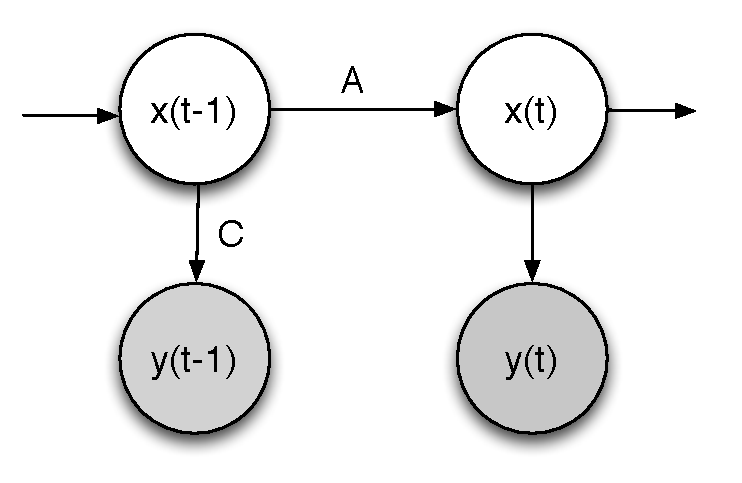
\includegraphics[width=0.4\textwidth]{d1.pdf}}

This time series model is imagined repeated for $t=1,\ldots,T$. It has \Blue{\emph{observations}} $y$ (shaded) for each time point and also \Blue{\emph{unobserved}} or \Blue{\emph{hidden}} or \Blue{\emph{latent variables}} $x$ and two sets of \Blue{\emph{parameters}} $A$ (for transitions) and $C$ (for emissions).\\[1ex]

To use the model we must decide what to do with all unobserved quantities. This is
broadly known as \Blue{\emph{learning}} or \Blue{\emph{training}} a model. Options include \Red{\emph{inference}}, \Red{\emph{estimation}}, \Red{\emph{sampling}} and \Red{\emph{marginalisation}}.\\[1ex]

Note, that the difference between \Blue{\emph{latent variables}} and \Blue{\emph{parameters}} is that the number latent variables grow with the number of observations (in this case, one for each time point), whereas the number of parameters remains constant.
\end{frame}


\begin{frame}
\frametitle{Practical modelling}

The specification of a model includes the complete structure as well as all assumptions (and priors) used as well as any pre-specified parameters. 

In practise, we need to be able to do the following tasks
\begin{itemize}
\item treat the unobserved quantities (training), including
\begin{itemize}
\item the latent variables
\item the parameters
\item possibly some aspects of the structure of the model
\end{itemize}
\item make predictions on test cases
\item interpret the trained model, what insights is the model providing?
\item evaluate the accuracy of model
\begin{itemize}
\item note: accuracy on the training and test sets may differ systematically
\end{itemize}
\item do model selection and model criticism: chose between different models, or between different variants of a model, what are limitations of the model?
\end{itemize}

All these tasks need to be solved either exactly or approximately, on a given budget
of computation and memory.
\end{frame}

\begin{frame}
\frametitle{A common misunderstanding}

The role of a model is to make predictions and provide insight into certain aspects of the data.\\[1ex]

The role of a model is \Red{\emph{not}} to be a complete description of all aspects of the data (only the data itself does this).\\[1ex]

From this perspective, it is clear that terms such as \Blue{\emph{true model}} or \Blue{\emph{correct model}} are \Red{\emph{meaningless}} in the context of machine learning.\\[2ex]

\emph{Essentially, all models are wrong, but some are useful.}\\
\hfill --- George E. T. Box
\end{frame}

\end{document}  